\section{Netzwerk}

\subsection{Allgemeine Definitionen}
\subsubsection{Datentypen}
Um hohe portabliltät zu gewährleisten verwenden wir nur sichere Datentypen.
Insbesondere gilt dies für Zahlen. Statt den Datentypen short, int, long verwenden
wir (u)int8\_t, (u)int16\_t, ....\\
Außerdem sollten immer Funktionen mit Längenbegrenzung benutzt werden, 
um Buffer-Overflows zu vermeiden.

\begin{figure}[ht!]
 \centering
 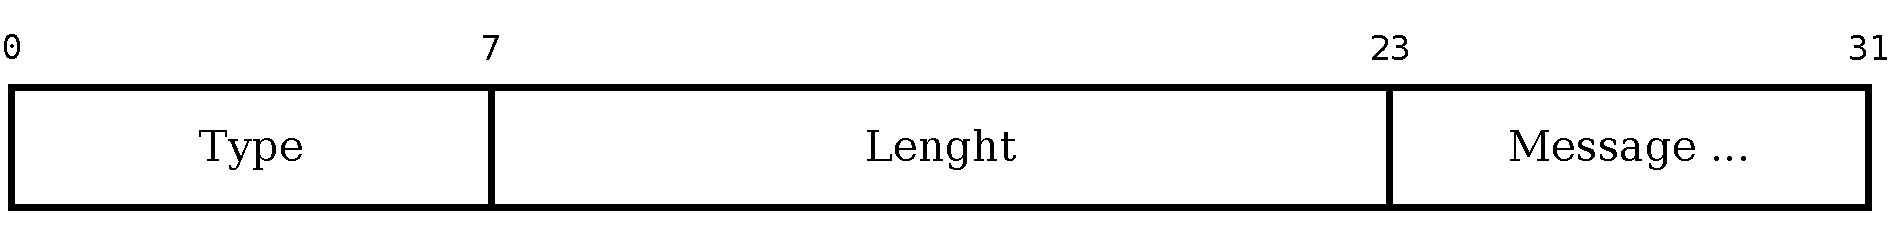
\includegraphics[width=\textwidth,keepaspectratio=true]{Bilder/header.pdf}
 \caption{Header}
 \label{Header}
\end{figure}

\subsubsection{Serialisierung}
Alle structs werden zum senden serialisiert in ein char-Array. \\
Der Server deserialisiert diesen String wieder.

\begin{lstlisting}
// PSEUDOCODE!
struct login_data {
    char name[50];
    uint8_t role;
}

// BUFFER
char buf[sizeof(login_data);

// SERIALISIEREN
strncpy(buf, login_data, sizeof(buf));

// DESERIALISIEREN
strncpy(login_data, buf, sizeof(login_data));
\end{lstlisting}

\subsubsection{Benutzerrollen}
\begin{lstlisting}
enum ROLE {
    Dozent = 1
    Tutor = 2
    Student = 3
};
\end{lstlisting}

\subsubsection{Schreib- und Leserecht}
Als Datentyp wird \code{uint8\_t} verwendet.
\begin{itemize}
	\item Modify 0 = nur lesend
	\item Modify 1 = schreibzugriff (exclusiv)
\end{itemize}

\subsubsection{Message-Types}
\begin{lstlisting}
enum M_TYPES {
    Login = 1,
    Quit, /*** eigentlich nicht nötig; Client bzw. Server */
          /*** schließt Verbindung einfach */
    Request,
    Shutdown,
    Release,
    Aquire,
    Modify,
    Clear,
    Status,
};
\end{lstlisting}

\subsection{Kommunikationsablauf}
Dieser Abschnitt spezifiziert den Austausch der einzelnen Datenstrukturen
über das Netzwerk.

Für die Beschreibung des Aufbaus der einzelnen Pakete: 
> siehe Abschnitt Datenstrukturen

\subsubsection{Login}
\begin{lstlisting}
Login       >>>
            <<<     Login
\end{lstlisting}

\subsubsection{Quit}
\begin{lstlisting}
*** eigentlich nicht nötig; Client bzw. Server schließt Verbindung einfach ***
\end{lstlisting}

\subsubsection{Request}
\begin{lstlisting}
Request     >>>
            <<<     Request (an Dozent)
# Bei Zustimmung des Dozenten die Schreibrechte abzugeben
Status      >>>
            <<<     Status (an anfragenden Client: Schreibrechte)
            <<<     Status (an alle Anderen: Tutor +1)
\end{lstlisting}

\subsubsection{Shutdown}
\begin{lstlisting}
Shutdown    >>>     (Server schließt alle Verbindungen)
\end{lstlisting}

\subsubsection{Release}
\begin{lstlisting}
Release     >>>
            <<<     Status (an releasing Client: nur Leserechte)
            <<<     Status (an Dozent: Schreibrechte)
            <<<     Status (an alle Anderen: Tutoren -1)
\end{lstlisting}

\subsubsection{Aquire}
\begin{lstlisting}
Aquire      >>>
            <<<     Status (an Client der aktuell schreibberechtig ist: nur lesend)
            <<<     Status (an Dozent: Schreibrechte)
            <<<     Status (an alle Anderen: Tutoren -1)
\end{lstlisting}

\subsubsection{Modify}
\begin{lstlisting}
Modify      >>>
            <<<     Modify (Änderungen an alle Clients verteilen)
\end{lstlisting}

\subsubsection{Clear}
\begin{lstlisting}
Clear       >>>
            <<<     Clear (an alle Clients: Tafel wurde gelöscht)
\end{lstlisting}

\subsubsection{Status}
\begin{lstlisting}
*** Ein eigener Status-Befehl existiert nicht. Status-Nachrichten
*** dienen als Bestätigung für bestimmte Befehle an den Client
*** und als Update für den Client-Status.
*** Für die Verwendung: siehe andere Befehle
\end{lstlisting}

\subsection{Datenstrukturen}
\begin{lstlisting}
#pragma pack(1)
struct HEADER {
    uint16_t size; /* Gesamtgröße in Bytes */
    uint8_t type; /* Wert aus M_TYPES */
};


/*
 * Packet:  Login
 *
 * Beschreibung:
 * Login-Versuch von Client bzw. Antwort von Server auf Login von Client.
 *
 *      >>> Richtung: Client > Server
 *      + "client_name" MUSS gesetzt und 0-terminiert sein und
 *        ist auf 25 Zeichen (inkl. O-Byte) begrenzt
 *      + "role" SOLLTE gesetzt sein, kann aber in jedem Fall vom
 *        Server geändert werden
 *
 *      >>> Richtung: Server > Client
 *      + "client_name" KANN gesetzt sein
 *      + wenn vorhanden muss dieser 0-terminiert sein und
 *        ist auf 25 Zeichen (inkl. 0-Byte) begrenzt
 *      + "role" MUSS gesetzt sein und MUSS vom Client respektiert werden
 *      + im Fehlerfall ist role == 0
 */
struct LOGIN {
    struct NET_HEADER header;
    char[25] client_name;
    uint8_t role; /* Wert aus ROLE */
};


/*
 * Packet:  Quit
 *
 * Beschreibung:
 * *** eigentlich nicht nötig; Client bzw. Server 
 * *** schließt Verbindung einfach
 *
 *      >>> Richtung: Server > Client
 *      + Keine Nutzdaten/Payload
 *      + Message Type in header ausreichend (kein "Payload Struct")
 */


/*
 * Packet:  Request
 *
 * Beschreibung:
 * Client fordert Schreibrechte an bzw. Anfrage an Dozent für Schreibrechte
 *
 *      >>> Richtung: Client > Server
 *      + "cid" wird nicht berücksichtigt
 *      + "client_name" KANN gesetzt sein
 *      + "client_name" muss 0-terminiert sein und ist auf 25 Zeichen
 *        begrenzt (inkl. 0-Byte)
 *
 *      >>> Richtung: Server > Client
 *      + "cid" MUSS gesetzt sein
 *      + "client_name" MUSS gesetzt sein
 *      + "client_name" MUSS 0-terminiert sein und ist auf 25 Zeichen
 *        begrenzt (inkl. 0-Byte)
 */
struct REQUEST {
    struct NET_HEADER header;
    uint8_t cid;
    char client_name[25];
};


/* 
 * Packet:  Shutdown
 *
 * Beschreibung:
 * System komplett beenden
 *
 *      >>> Richtung: Client > Server
 *      + Keine Nutzdaten/Payload
 *      + Message Type in header ausreichend (kein "Payload Struct")
 */


/*
 * Packet:  Release
 *
 * Beschreibung:
 * Schreibrechte an Dozent zurückgeben
 *
 *      >>> Richtung: Client > Server
 *      + Keine Nutzdaten/Payload
 *      + Message Type in header ausreichend (kein "Payload Struct")
 */


/*
 * Packet:  Aquire
 *
 * Beschreibung:
 * Aktuellem Benutzer Schreibrechte entziehen
 *
 *      >>> Richtung: Client > Server
 *      + Keine Nutzdaten/Payload
 *      + Message Type in header ausreichend (kein "Payload Struct")
 *
 */


/*
 * Packet:  Modify
 *
 * Beschreibung:
 * Änderungen an der Tafel übertragen
 *
 *		>>> Richtung: Client > Server
 *      + "cid" MUSS gesetzt sein
 *      + "board" MUSS gesetzt sein, ist 0-terminiert und max. 1200 Zeichen (inklusive 0-Byte)
 *
 *      >>> Richtung: Server > Client
 *      + "cid" wird nicht berücksichtigt
 *      + "board" MUSS gesetzt sein, ist 0-terminiert und max. 1200 Zeichen (inklusive 0-Byte)
 */
struct MODIFY {
    struct NET_HEADER header;
    uint8_t cid;
    char board[1200];
};


/*
 * Packet:  Clear
 *
 * Beschreibung:
 * Löschen des Tafelinhalts
 *
 *      >>> Richtung: Client > Server
 *      + Keine Nutzdaten/Payload
 *      + Message Type in header ausreichend (kein "Payload Struct")
 */


/*
 * Packet:  Status
 *
 * Beschreibung:
 * Änderung des Status im Server bzw. Client
 *
 *      Richtung: Client > Server (als Antwort auf 'Request'
 *      + "client_name" KANN gesetzt sein (vom Server nicht berücksichtigt)
 *      + "cid" MUSS gesetzt sein
 *      + restliche Elemente KÖNNEN gesetzt sein,
 *        aber vom Server nicht weiter berücksichtigt
 *
 *      Richtung: Server > Client
 *      + "client_name" MUSS gesetzt sein
 *      + "role" KANN gesetzt sein
 *      + "cid" KANN gesetzt sein
 *      + "write" MUSS entweder 1 = schreibender, oder 0 = lesender
 *        Zugriff sein
 *      + "nof_doz" (Anzahl angemeldeter Dozenten) KANN gesetzt sein
 *        und ist entweder 0 oder 1 (nicht mehr als 1 Dozent möglich)
 *      + "nof_tut" (Anzahl Tutoren) KANN gesetzt sein und ist
 *        entweder 0 oder 1 (Student ist nur Tutor, wenn er schreibrechte hat)
 *      + "nof_std" (Anzahl angemeldeter Studenten) KANN gesetzt sein
 */
struct STATUS {
    struct NET_HEADER header;
    char client_name[25];
    uint8_t role;
    uint32_t cid;
    unit8_t write;
    uint8_t nof_doz;
    uint8_t nof_tut
    uint32_t nof_std;
}

#pragma pack(0)
\end{lstlisting}
